\section{Техническое задание}
\subsection{Основание для разработки}

Основанием для разработки является задание на выпускную квалификационную работу бакалавра <<\Тема {} \ТемаВтораяСтрока>>.

\subsection{Цель и назначение разработки}

Основной задачей выпускной квалификационной работы является разработка платформы для создания компьютерных изометрических ролевых игр с заранее отрисованным двумерным фоном и спрайтовыми персонажами для продвижения популярности рпг-игр».

Данный программный продукт предназначен для демонстрации практических навыков, полученных в течение обучения.

Задачами данной разработки являются:
\begin{enumerate}
\item Анализ существующих ролевых игр.
\item Разработка концептуальной модели ролевых игр.
\item Проектирование программной системы для создания ролевых игр.
\item Реализация программной системы для создания ролевых игр.
\item Тестирование разработанной системы.
\end{enumerate}

\subsection{Требования пользователя к платформе}

Платформа должна включать в себя:
\begin{itemize}
    \item создание зон;
    \item создание объектов;
    \item создание персонажей;
    \item добавление объектов в зону;
    \item удаление объектов из зоны;
    \item реализацию сценариев.
\end{itemize}

Композиция шаблона игры, созданной на движке, представлена на рисунке ~\ref{maket:image}.

\begin{figure}[ht]
	
\includegraphics[width=1\linewidth]{maket}
	\caption{Композиция шаблона интерфейса игры}
	\label{maket:image}
\end{figure}
%\vspace{-\figureaboveskip} % двойной отступ не нужен (можно использовать, если раздел заканчивается картинкой)

\subsection{Описание платформы для создания RPG игр}
Клиент создает модуль содержащий методы модуля RPGGame, например bggame. В этом модуле мы создаем мир игры, с помощью new\_actor. Мы можем вызывать их много раз с разными параметрами, или загрузить параметры для этих функций из файла. После чего у нас есть персонажи и предметы. Мир также состоит из зон (Area). Каждая зона включает в себя графику, персонажи и предметы и сценарии взаимодействия. Исключение составляет команда PC, которая может перемещаться из зоны в зону (это мы программируем у клиента). Команду мы тоже определяем стартовую и впоследствии можем менять (add\_actor\_to\_team, remove\_actor\_from\_team). Каждому персонажу и объекту может соответствовать пользовательский сценарий (он активируется при нажатии мышкой на объект). Сценарий может включать диалог, взятие предмета, добавление персонажа в команду, квест и т.д.
Зона тоже может содержать сценарий, который запускается когда команда попадает в зону.
Клиентский класс (BGGame) также содержит глобальные переменные, определяющие ситуации в игре (например квесты). Локальные переменные могут быть в зоне.

Как программируются зоны. Если нужны локальные переменные (состояние локальных событий), то тогда нужно создавать класс своей зоны как наследник от Area. Или же просто использовать класс Area. Добавляем зону в игру new\_area(name, area). Переключаем зону - set\_area(name). Глобальные сценарии находятся в классе игры (BGGame), мы подключаем их как :
Area.set\_enter\_script(script)
В зону мы добавляем персонажей и предметы как add\_object(x,y, obj) - z не нужно, так как слой можно определить по y координате.
В конкретную зону мы добавляем сценарий для взаимодействия как: Game.game.start\_script(script, name)
Как происходит переход команды между зонами.
В зоне определяем объект дверь, по клику мыши она может открываться и закрываться (меняется состояние объекта). Назначаем сценарий walk\_script(script), который срабатывает когда кто-то из команды пересекает объект. В этом сценарии мы меняем зону на нужную (set\_area), и устанавливаем команду в нужную позицию (set\_team). В другой зоне делается аналогично, только переход и позиция будут другими.
Сценарии - это потоки которые запускаются параллельно (метод RPGGame.start\_script(script)). Сценарий может быть остановлен (stop\_script(name)).
Таким образом, мир будет интерактивным.
Как связано окно и графика с игрой. В окне мы делаем таймер, который вызывает метод update нашей игры (BGGame). Этот метод выполняет все действия объектов в игре за 1 кадр времени.
Также в таймере вызываем Graphics.update(), который обновляет графику игры.
Все объекты (Actor, Item) должны иметь состояния (как минимум одно). Каждое состояние связано с спрайтом (или анимацией). То есть переключение состояния меняет графику объекта.

А вообще сценарии и глобальные переменные могут быть без классов, а просто в модулях, так проще, чтобы к ним был доступ из всех комнат. Тогда и функции движка должны быть доступны везде (то есть во всех сценариях). Например делаем модуль руины (ruins) представлен на рисунке \ref{ruins:image}:
\begin{figure}[H]
	\begin{lstlisting}[language=Python]
		import random
		from math import sqrt
		import time
		from rpg.area import *
		from rpg.sprite import *
		from rpg.rectangle import *
		from rpg.game import Game
		from rpg.portal import Portal
		
		class Ruins(Area):
			def __init__(self):
				'''
				Класс игровой зоны Ruins
				
				'''
				super().__init__()
				self.add_sprite(Sprite('images/fon3.png'), 590, 400, 0)
				self.add_rect(Rectangle(x=0, y=0, width=Sprite('images/fon3.png').image.width(), height=Sprite('images/fon3.png').image.height()))
				from grunt import Grunt
				self.grunt = Grunt(0,0,0)
				from footman import Footman
				self.footman = Footman(0,0,0)
				self.add_object(self.footman, 120, 620, 1)
				self.add_object(self.grunt, 500, 685, 1)
				p = Portal(400, 400, 200, 200, 'Village', 480, 100)
				self.add_object(p, p.pos_x, p.pos_y, 100)
				#Game.game.start_script(self.walk, "grunt", 50, 50)
				Game.game.start_script(self.ai, "ai", self.grunt)
				Game.game.start_script(self.walk_two, "footman", 50, 50)
\end{lstlisting}  
\caption{Пример создания игровой зоны Ruins}
\label{ruins:image}
\end{figure}
Продолжение на рисунке \ref{ruins5:image}:
\begin{figure}[H]
	\begin{lstlisting}[language=Python]	
		def walk(self, step_x, step_y, actor):
			'''
			Сценарий для движения бугая
			
			:param step_x: шаг движения x
			:param step_y: шаг движения y
			'''
			if actor.hp <= 0:
				Game.game.stop_script("grunt")
			new_x = 300
			new_y = 500
			actor.is_attack = False
			# Выбираем случайное направление
			direction = random.choice(["up", "down", "left", "right"])
			
			# Устанавливаем целевую точку в зависимости от направления
			if direction == "up":
				new_y -= step_y
				new_x = step_x
			elif direction == "down":
				new_y += step_y
				new_x = step_x
			elif direction == "left":
				new_y = step_y
				new_x -= step_x
			elif direction == "right":
				new_y = step_y
				new_x += step_x
			
			# Обновляем координаты бугая
			actor.search_position(new_x, new_y)
			
			# Ждем 2 секунды перед выбором нового направления
			time.sleep(2)
	\end{lstlisting}  
	\caption{Пример создания игровой зоны Ruins}
	\label{ruins5:image}
\end{figure}
Продолжение на рисунке \ref{ruins2:image}:
\begin{figure}[H]
	\begin{lstlisting}[language=Python]		
		модуль bggame:
		from ruins import *
		import time
		import random
		
		class BaldursGame(Game):
			def __init__(self, canvas, window, **params):
			'''
			Класс конкретной игры для демонстрации
		
			:param canvas: класс графической системы
			:param window: окно на которое будет выводится игра
			'''
			super().__init__(canvas, window, **params)
			from mage import Mage
			self.add_pc_to_team(Mage(0, 0, 0))
			self.new_area('Ruins', Ruins())
			self.set_area('Ruins')
			self.set_team(500, 300, 100)
			self.timer()
	\end{lstlisting}  
	\caption{Пример создания игровой зоны Ruins}
	\label{ruins2:image}
\end{figure}


\subsubsection{Пример клиентского кода игры}
\paragraph{Cоздание классов персонажей/предметов}
Клиент создает модуль содержащий методы модуля RPGGame, например BaldursGateGame. В этом модуле клиент создает мир игры, с помощью new\_actor.
Пример представлен на рисунке \ref{answer:image}:
\begin{figure}[H]
	\begin{lstlisting}[language=Python]
		модуль bggame:
		from ruins import *
		import time
		import random
		
		class BaldursGame(Game):
			def __init__(self, canvas, window, **params):
			'''
			Класс конкретной игры для демонстрации
		
			:param canvas: класс графической системы
			:param window: окно на которое будет выводится игра
			'''
			super().__init__(canvas, window, **params)
			from mage import Mage
			self.add_pc_to_team(Mage(0, 0, 0))
			self.new_area('Ruins', Ruins())
			self.set_area('Ruins')
			self.set_team(500, 300, 100)
			self.timer()
	\end{lstlisting}  
\caption{Пример создания персонажа Mage}
\label{answer:image}
\end{figure}


\paragraph{Задание правил атаки}
Пользователь создаёт класс ADnDActor, наследник от класса Actor в своём модуле bggame, в нём он прописывает свои правила по которым происходит атака. То есть Actor.attack(self, actor), где actor - кого атакуют.
Пример представлен на рисунке \ref{attack:image}:
\begin{figure}[H]
	\begin{lstlisting}[language=Python]
		модуль adnd_actor:
		from math import sqrt
		from rpg.actor import Actor
		from rpg.animation import Animation
		import rpg.game
		import time
		
		class Adnd_actor(Actor):
		
			ATTACK_RANGE = 50
		
			def __init__(self, x, y, z, **params):
				super().__init__(x, y, z, **params)
				self.on_click = self.click
			
			def click(self):
				pc = rpg.game.Game.game.team_of_pc[0]
				if pc == self:
					return
				dx = pc.pos_x - self.pos_x
				dy = pc.pos_y - self.pos_y
				dist = sqrt(dx * dx + dy * dy)
				if dist <= self.ATTACK_RANGE:
					pc.is_attack = True
					pc.attack(self)
					time.sleep(0.125)
				if self.hp <=0:
					pc.is_attack = False
		
			def attack(self, actor):
				actor.hp -= self.damage
			def update(self):
				super().update()
				if self.hp <= 0:
					self.stop_move()
					self.set_state('death')
\end{lstlisting}  
\caption{Пример задания правил атаки персонажа}
\label{attack:image}
\end{figure}

\paragraph{Создание зон, заполнение их персонажами/объектами}
Мир также состоит из зон (Area). Каждая зона включает в себя графику, персонажи и предметы и сценарии взаимодействия. Исключение составляет команда PC, которая может перемещаться из зоны в зону (это мы программируем у клиента). Как программируются зоны. Если нужны локальные переменные (состояние локальных событий), то тогда нужно создавать класс своей зоны как наследник от Area. Или же просто использовать класс Area. Добавляем зону в игру new\_area(name, area). Переключаем зону - set\_area(name). Так же требуется задать область движения, её проще сделать как совокупность прямоугольников, за которые персонажи не могут выйти. Эти прямоугольники должны касаться друг друга, но не пересекаться. Тогда алгоритм проверки выхода несложный: выход за пределы области только тогда, когда прямоугольник персонажа пересек сторону (одну или две) одного из прямоугольников области, эта сторона не является касательной.
Пример представлен на рисунке \ref{area:image}:
\begin{figure}[H]
	\begin{lstlisting}[language=Python]
		from rpg.game import Game
		from rpg.portal import Portal
		
		class Ruins(Area):
			def __init__(self):
				super().__init__()
				self.add_sprite(Sprite('images/fon3.png'), 590, 400, 0)
				self.add_rect(Rectangle(x=0, y=0, width=Sprite('images/fon3.png').image.width(), height=Sprite('images/fon3.png').image.height()))
				from grunt import Grunt
				self.grunt = Grunt(0,0,0)
				from footman import Footman
				self.footman = Footman(0,0,0)
				self.add_object(self.footman, 120, 120, 1)
				self.add_object(self.grunt, 500, 185, 1)
				p = Portal(400, 400, 200, 200, 'Village', 480, 100)
				self.add_object(p, p.pos_x, p.pos_y, 100)
				Game.game.start_script(self.ai, "ai", self.grunt)
				Game.game.start_script(self.walk_two, "footman", 50, 50)		
	\end{lstlisting}  
\caption{Пример создания зоны Ruins}
\label{area:image}
\end{figure}
Продолжение на рисунке \ref{area2:image}:
\begin{figure}[H]
	\begin{lstlisting}[language=Python]	
		def walk(self, step_x, step_y, actor):
		'''
		Сценарий для движения бугая
		
		:param step_x: шаг движения x
		:param step_y: шаг движения y
		'''
		if actor.hp <= 0:
		Game.game.stop_script("grunt")
		new_x = 300
		new_y = 500
		actor.is_attack = False
		# Выбираем случайное направление
		direction = random.choice(["up", "down", "left", "right"])
		
		# Устанавливаем целевую точку в зависимости от направления
		if direction == "up":
		new_y -= step_y
		new_x = step_x
		elif direction == "down":
		new_y += step_y
		new_x = step_x
		elif direction == "left":
		new_y = step_y
		new_x -= step_x
		elif direction == "right":
		new_y = step_y
		new_x += step_x
		
		# Обновляем координаты бугая
		actor.search_position(new_x, new_y)
		
		# Ждем 2 секунды перед выбором нового направления
		time.sleep(2)
	\end{lstlisting}  
	\caption{Пример создания игровой зоны Ruins}
	\label{area2:image}
\end{figure}
\paragraph{Пример сценариев: переход между зонами}
Глобальные сценарии находятся в классе игры (BGGame), мы подключаем их как
Area.set\_enter\_script(script)
Как происходит переход команды между зонами.
В зоне определяем объект портал, по клику мыши когда персонаж заходит внутрь портала срабатывает self.actor\_in(self, actor). При создании портала, мы указываем кудаи в какую зону разместить команду персонажей.
Пример представлен на рисунке \ref{portal:image}:
\begin{figure}[H]
	\begin{lstlisting}[language=Python]
		from rpg.object import Object
		from rpg.game import Game
		from rpg.rectangle import Rectangle	
		class Portal(Object):
			def __ini__(self, x, y, width, height, area, team_x, team_y):
				self.states = None
				self.sprite = None
				self.category = 'portal'
				super().__init__(x, y, 0)
				self.rectangle = Rectangle(x, y, width, height)
				self.area = area
				self.team_x = team_x
				self.team_y = team_y
				self.visible = False
			
			def actor_in(self, actor):
				if actor.category == "pc":
					Game.game.set_area(self.area)
					Game.game.set_team(self.team_x, self.team_y, 100)
				actor.stop_move()		
		модуль ruins
		import random
		from math import sqrt
		import time
		from rpg.area import *
		from rpg.sprite import *
		from rpg.rectangle import *
		from rpg.game import Game
		from rpg.portal import Portal
		class Ruins(Area):
			def __init__(self):
				super().__init__()
				self.add_sprite(Sprite('images/fon3.png'), 590, 400, 0)
				self.add_rect(Rectangle(x=0, y=0, width=Sprite('images/fon3.png').image.width(), height=Sprite('images/fon3.png').image.height()))
				from grunt import Grunt
				self.grunt = Grunt(0,0,0)
				from footman import Footman
				self.footman = Footman(0,0,0)
				self.add_object(self.footman, 120, 120, 1)
				self.add_object(self.grunt, 500, 185, 1)
				p = Portal(400, 400, 200, 200, 'Village', 480, 100)
	\end{lstlisting}  
	\caption{Пример перехода между зонами}
	\label{portal:image}
\end{figure}

\paragraph{Как будет идти бой}
Бой будет совершаться с помощью сценариев. У класса Adnd\_actor есть метод attack(self, actor), который уменьшает текущее количество здоровья у actor. В модуле game существуют методы start\_script(script, name), stop\_script(name). С помощь сценариев возможно запускать параллельные потоки. В конкретную зону будет добавляться сценарий 'ai', в который передаётся конкретный персонаж. В этом сценарии указывается поведение противника, Что он должен сближаться с персонажем игрока, и когда расстояние до атаки будет достаточным, чтобы её совершить, будет вызван метод actor.attack. Для того, чтобы пользователь мог атаковать персонажа, у каждого экземпляра класса adnd\_actor есть метод click(self), который вызывает проверку условия, если персонаж близко к персонажу игрока, хранящемуся в rpg.game.Game.team\_of\_pc, то вызвать у pc=rpg.game.Game.team\_of\_pc[0], attack(self).
Пример представлен на рисунке \ref{battle:image}:
\begin{figure}[H]
	\begin{lstlisting}[language=Python]
		модуль adnd_actor:
		from math import sqrt
		from rpg.actor import Actor
		from rpg.animation import Animation
		import rpg.game
		import time
		class Adnd_actor(Actor):	
			ATTACK_RANGE = 50
			def __init__(self, x, y, z, **params):
				super().__init__(x, y, z, **params)
				self.on_click = self.click
			def click(self):
				pc = rpg.game.Game.game.team_of_pc[0]
				if pc == self:
					return
				dx = pc.pos_x - self.pos_x
				dy = pc.pos_y - self.pos_y
				dist = sqrt(dx * dx + dy * dy)
				if dist <= self.ATTACK_RANGE:
					pc.is_attack = True
						pc.attack(self)
						time.sleep(0.125)
				if self.hp <=0:
					pc.is_attack = False
			def attack(self, actor):
				actor.hp -= self.damage
			def update(self):
				super().update()
				if self.hp <= 0:
					self.stop_move()
					self.set_state('death')
\end{lstlisting}  
\caption{Пример задания боя между персонажами}
\label{battle:image}
\end{figure}
Продолжение на рисунке \ref{battle2:image}:
\begin{figure}[H]
	\begin{lstlisting}[language=Python]
		модуль ruins
		import random
		from math import sqrt
		import time
		from rpg.area import *
		from rpg.sprite import *
		from rpg.rectangle import *
		from rpg.game import Game
		from rpg.portal import Portal
		class Ruins(Area):
			def __init__(self):
				super().__init__()
				self.add_sprite(Sprite('images/fon3.png'), 590, 400, 0)
				self.add_rect(Rectangle(x=0, y=0, width=Sprite('images/fon3.png').image.width(), height=Sprite('images/fon3.png').image.height()))
				from grunt import Grunt
				self.grunt = Grunt(0,0,0)
				from footman import Footman
				self.footman = Footman(0,0,0)
				self.add_object(self.footman, 120, 120, 1)
				self.add_object(self.grunt, 500, 185, 1)
				p = Portal(400, 400, 200, 200, 'Village', 480, 100)
				self.add_object(p, p.pos_x, p.pos_y, 100)
				Game.game.start_script(self.ai, "ai", self.grunt)
				Game.game.start_script(self.walk_two, "footman", 50, 50)	
			def ai(self, actor):
				if actor.hp <= 0:
					Game.game.stop_script("ai")
				import rpg.game
				pc = rpg.game.Game.game.team_of_pc[0]
				new_x = pc.pos_x
				new_y = pc.pos_y
				
				actor.search_position(new_x, new_y)
				dx = pc.pos_x - actor.pos_x
				dy = pc.pos_y - actor.pos_y
				dist = sqrt(dx * dx + dy * dy)
				if dist <= actor.ATTACK_RANGE:
					actor.is_attack = True
					actor.attack(pc)
					time.sleep(1)
					if pc.hp <=0:
						actor.update()
						Game.game.stop_script("ai")
				else:
					actor.is_attack = False
				time.sleep(2)
\end{lstlisting}  
\caption{Пример задания боя между персонажами}
\label{battle2:image}
\end{figure}

\subsection{Особенности Dungeons and Dragons}
Dungeons and Dragons (DnD) - это настольная ролевая игра, в которой игроки сотрудничают вместе, чтобы создать историю в фантастическом мире. В DnD один игрок выступает в роли Мастера игры (Мастера подземелий), который рассказывает и контролирует мир, а остальные игроки играют за своих персонажей, которых они создают и развивают.
Основные элементы ролевой системы DnD включают:
	\begin{enumerate} 
		\item Классы и расы. Классы представляют различные роли и специализации персонажей, такие как воин, маг, жрец. Каждый класс имеет свои уникальные способности и навыки.
			
				Особенности воина -- воин специализируется на ближнем бою, может использовать все виды оружия, может носить все доспехи и щиты, не способен накладывать заклинания, его кость здоровья 10-гранный кубик (D10).
				 Особенности мага -- маг специализируется на дальнем бою, может использовать только боевые посохи и короткие мечи, не может носить доспехи , способен накладывать заклинания, наносящие большое количество урона, его кость здоровья 6-гранный кубик (D6).
				Особенности жреца -- жрец специализируется на ближнем бою, может использовать простое оружия, может носить лёгкие,средние доспехи и щиты, способен накладывать заклинания, исцеляющие его, его кость здоровья 8-гранный кубик (D8).
			
		\item Расы определяют происхождение персонажа и дают особые характеристики и способности. Примеры рас включают эльфов, дварфов, людей.
			
			 Особенности человека -- человек на старте получает +1 ко всем характеристикам, его размер средний.
			 Особенности эльфа -- эльф получает +2 к ловкости и +1 к мудрости, его размер средний, у эльфа есть тёмное зрение в радиусе 30 футов.
			 Особенности дварфа -- дварф получает +2 к силе и +2 к телосложению, его размер маленький, у дварфа есть тёмное зрение в радиусе 30 футов.
			
		\item Характеристики.
			Характеристики определяют физические и умственные способности персонажа, такие как сила, ловкость, телосложение, интеллект, мудрость, харизма. Они влияют на способности и успех персонажа в различных ситуациях.
			Сила -- характеристика влияющая на броски атак рукопашным оружием, а так же на проверки навыков: атлетика.
			 Ловкость -- характеристика влияющая на броски атак совершаемых стрелковым оружием, на класс доспеха персонажа, а так же на проверки навыков: акробатика, ловкость рук, скрытность.
			Телосложение -- характеристика влияющая на колличество здоровья персонажа.
			Интеллект -- характеристика влияющая на броски атак совершённых заклинаниями волшебника, а так же на проверки навыков: магия, история, природа, расследование, религия.
			 Мудрость -- характеристика влияющая на броски атак  совершённых заклинаниями жреца, а так же на проверки навыков: восприятие, выживание, проницательность, уход за животными, медицина.
			 Харизма -- характеристика влияющая на общение с не игровыми персонажами, а так же на проверки навыков: выступление, убеждение, обман, запугивание.
		\item Навыки. Навыки представляют специализации персонажа в определенных областях, таких как взлом замков, обращение с оружием, магия и т.д. Навыки могут быть использованы для выполнения действий и решения задач
		\item Броски костей.
			 Игра DnD использует различные виды игровых костей для случайной генерации результатов. Например, для определения успеха атаки или проверки навыка игрок может бросить 20-гранный кубик (D20) и добавить соответствующие модификаторы.
		\item Приключения и задания.
			 Мастер игры создает историю, включающую задания и приключения, которые игроки выполняют. Задания могут включать исследование подземелий, сражение с монстрами, решение головоломок и взаимодействие с неигровыми персонажами.
		\item Прогрессия и опыт.
			Персонажи получают опыт за выполнение заданий и сражение с врагами. Зарабатывая опыт, персонажи повышают уровень, получают новые способности и становятся сильнее.
		\item Магия.
			DnD имеет разветвленную систему магии, позволяющую персонажам использовать заклинания различных уровней и школ. Магические заклинания могут влиять на бой, лечение, обнаружение и другие аспекты игры.
	\end{enumerate}
\subsection{Пример игры}
Создаётся рабочее окно tkinter, на нём пользователь видит текущую зону, из зоны current\_area, так же все объекты, находящиеся в ней, и всех персонажей из команды персонажей, текущей игры. Пользователь может взаимодействовать с окном с помощью мыши. Левым кликом мыши по окну вызывает метод mouse\_click у текущей игры. который вызывает проверку находится ли в координатах, в которых был совершён клик, какой-либо персонаж или объект, и если есть, то вызвать метод on\_click. Если персонажа в данных координатах нет, то вызвать у всех персонажей с полем category == "pc" метод search\_position(x,y), который указывает координаты движения, которые должны прийти персонажи. Так же работают все сценарии, конкретной зоны. они работают до тех пор, пока не будет вызвано условие останавливающее, конкретный сценарий.
На рисунке ~\ref{prec:image} сформированы следующие действия пользователя и их последствия.
\begin{figure}[H]
	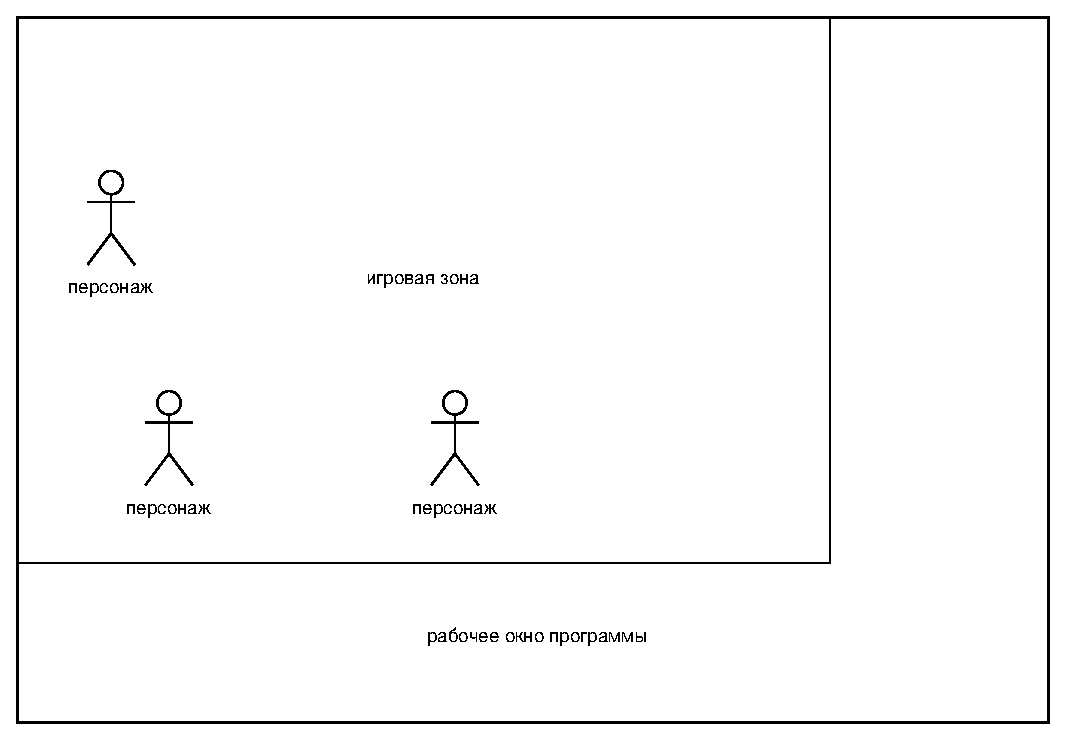
\includegraphics[width=1\linewidth]{prec}
	\caption{Шаблон игры}
	\label{prec:image}
\end{figure}
%\vspace{-\figureaboveskip} % двойной отступ не нужен (можно использовать, если раздел заканчивается картинкой)

\subsection{Требования к оформлению документации}

Разработка программной документации и программного изделия должна производиться согласно ГОСТ 19.102-77 и ГОСТ 34.601-90. Единая система программной документации.
Программная документация должна включать в себя:
\begin{itemize}
	\item техническое задание;
	\item технический проект;
	\item рабочий проект.
\end{itemize}